\subsection{Back-End}
	\subsubsection*{Informazioni sul package}
		\begin{figure}[h]
			\centering
			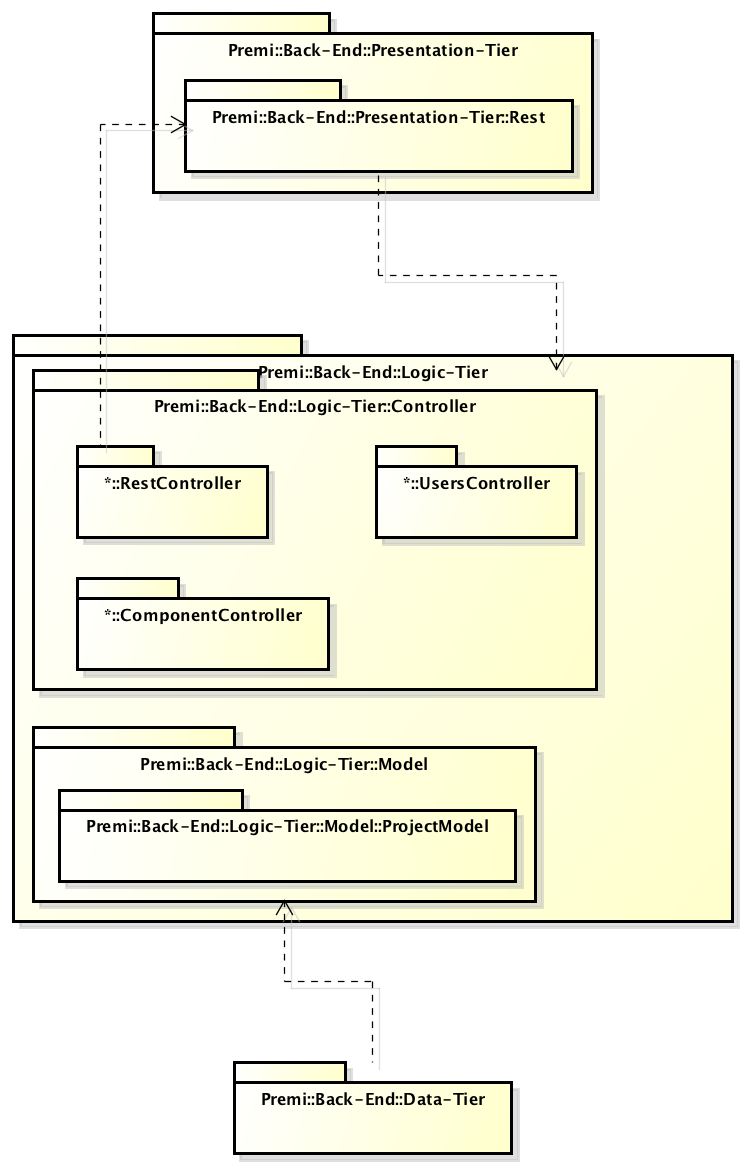
\includegraphics[width=0.9\linewidth]{img/back-end_package}
			\caption[Premi::Back-End]{Premi::Back-End}
		\end{figure}
		Il package contiene le componenti della parte di \gls{back-end} dell'applicazione.
		
	\subsubsection*{Package contenuti}
		\begin{itemize}
			\item Premi::Presentation-Tier;
			\item Premi::Http;
			\item Premi::Model;
			\item Premi::Data-Tier.
		\end{itemize}

\newpage

\subsection{Premi::Presentation-Tier}
	\subsubsection*{Informazioni sul package}
		\begin{figure}[h]
			\centering
			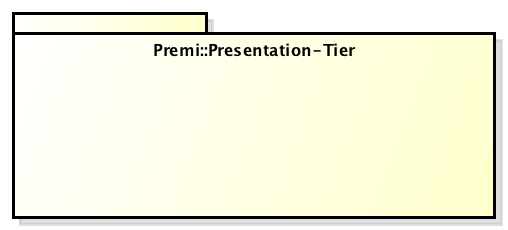
\includegraphics[width=0.5\linewidth]{img/premi_presentation-tier}
			\caption[Premi::Presentation-Tier]{Premi::Presentation-Tier}
		\end{figure}
		Il package contiene rende possibile l'interfacciamento con il \gls{front-end}. Comunica con altri livelli attraverso i risultati di output al livello browser/client e tutti gli altri livelli della rete.
		
		
\newpage
		
\subsection{Logic Tier}
	\begin{figure}[h]
		\centering
		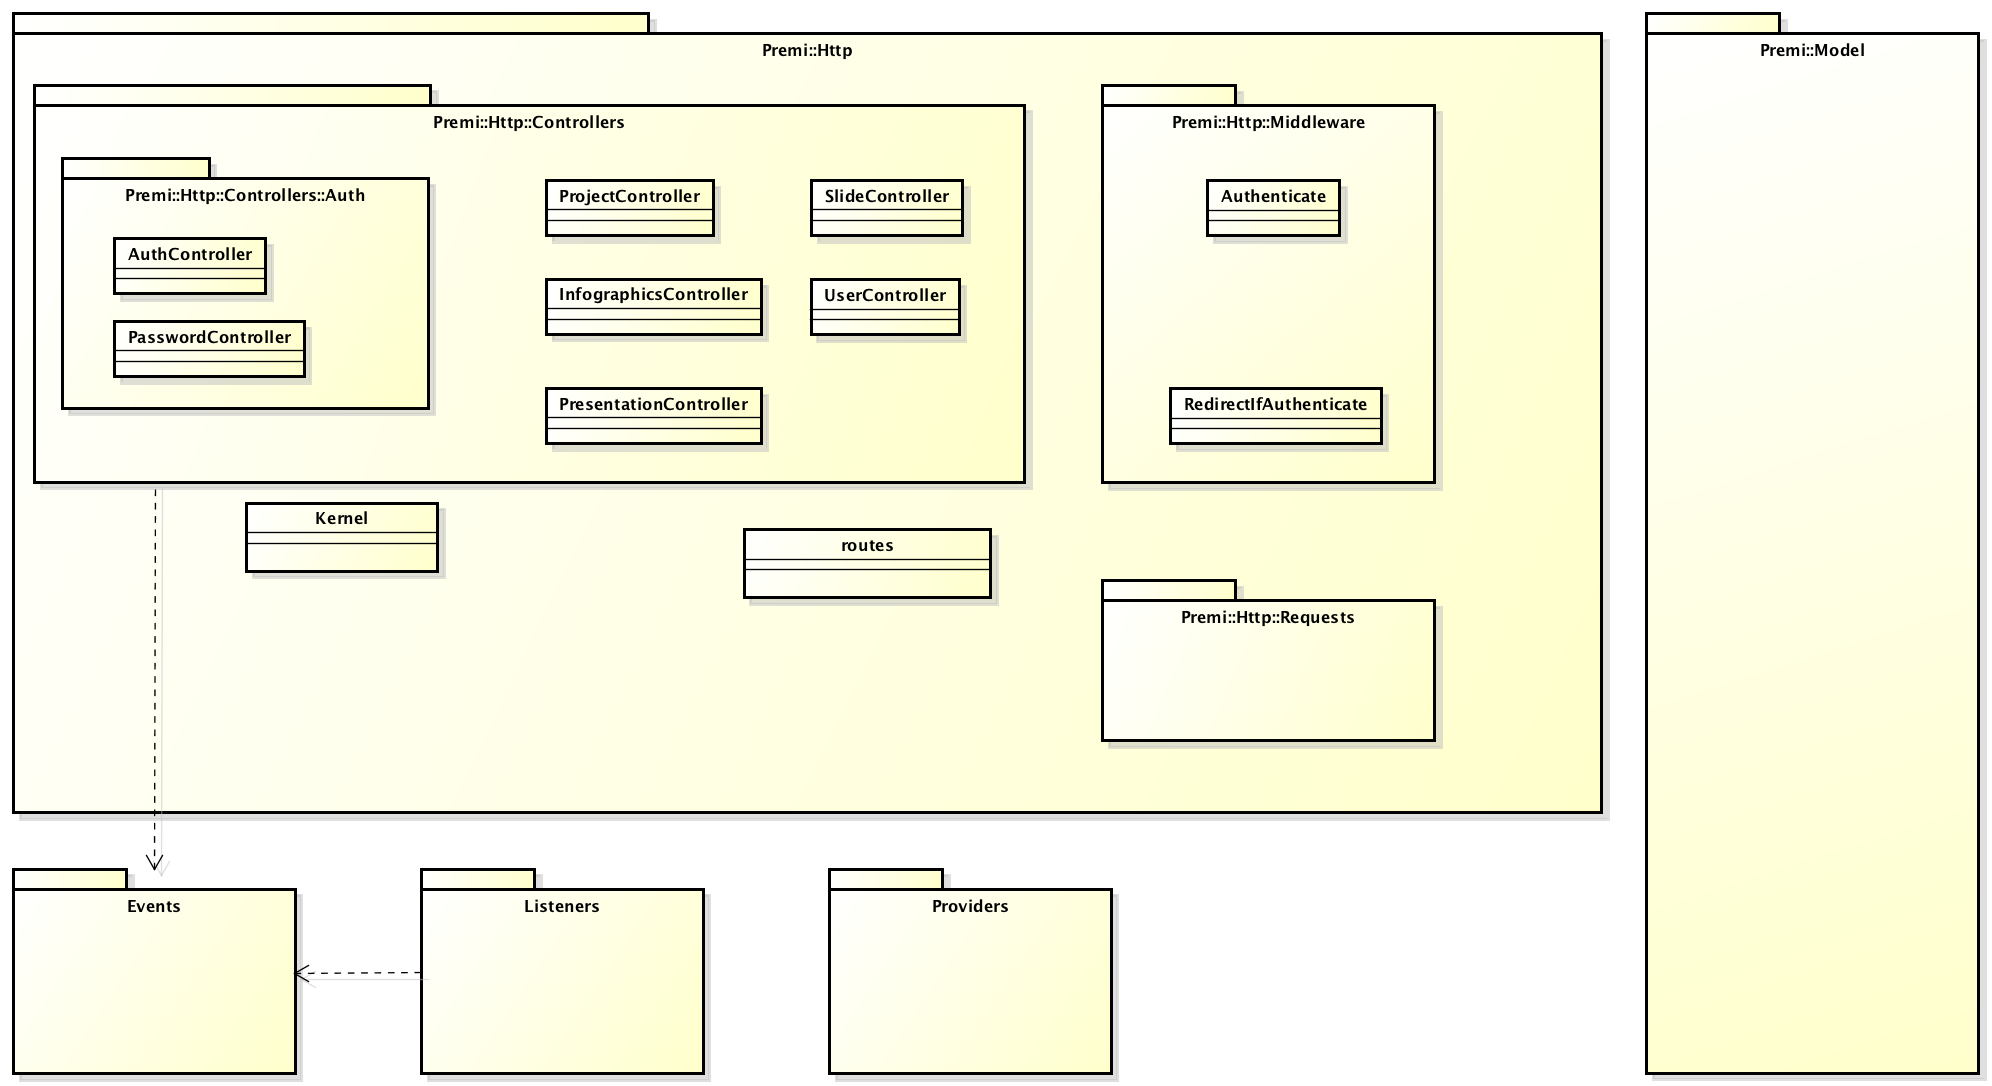
\includegraphics[width=\linewidth]{img/back-end_logic-tier_package}
		\caption[Premi::Http , Premi::Model]{Premi::Http , Premi::Model}
	\end{figure}
	Il core dell'applicazione viene implementato dal Model, che incapsulando lo stato dell'applicazione definisce i dati e le operazioni che possono essere eseguite su questi. Il package Http contiene Il componente Controller che ha la responsabilità di trasformare le interazioni dell'utente in azioni eseguite dal Model.
	
	\subsubsection*{Package contenuti}
	\begin{itemize}
		\item Premi::Http;
		\item Premi::Model.
	\end{itemize}

\newpage
\subsection{Premi::Http}
		\begin{figure}[h]
			\centering
			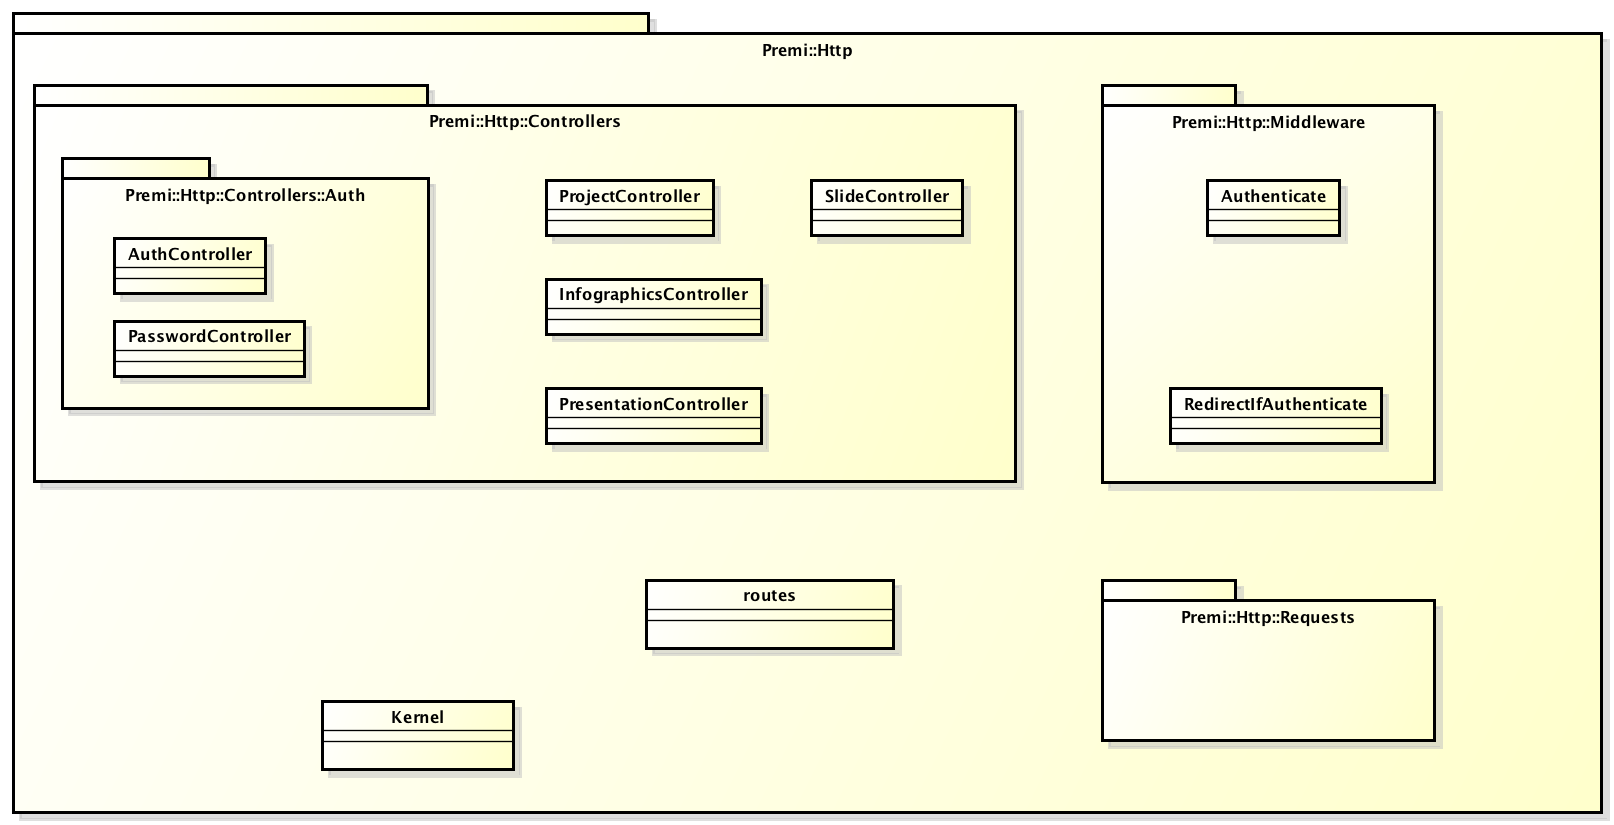
\includegraphics[width=0.9\linewidth]{img/premi_http}
			\caption[Premi::Http]{Premi::Http}
			\label{fig:premi_http}
		\end{figure}

	\subsubsection*{Informazioni sul package}
	 Il logic tier contiene a sua volta svariati package. Il package Http funziona come un'interfaccia alla vera applicazione.
	 \subsubsection*{Classi contenute}
	 \begin{itemize}
	 	\item \textbf{routes: }collega una specifica richiesta ad un set di istruzioni ben precise;
	 	\item \textbf{Kernel: }"filtro" attraverso cui passano tutte le richieste.
	 \end{itemize}
	 \subsubsection*{Package contenuti}
		 \begin{itemize}
		 	\item Premi::Http::Controllers;
		 	\item Premi::Http::Middleware;
		 	\item Premi::Http::Request;
		 \end{itemize}

\newpage
\subsection{Premi::Http::Controllers}
	\subsubsection*{Informazioni sul package}
	\begin{figure}[h]
		\centering
		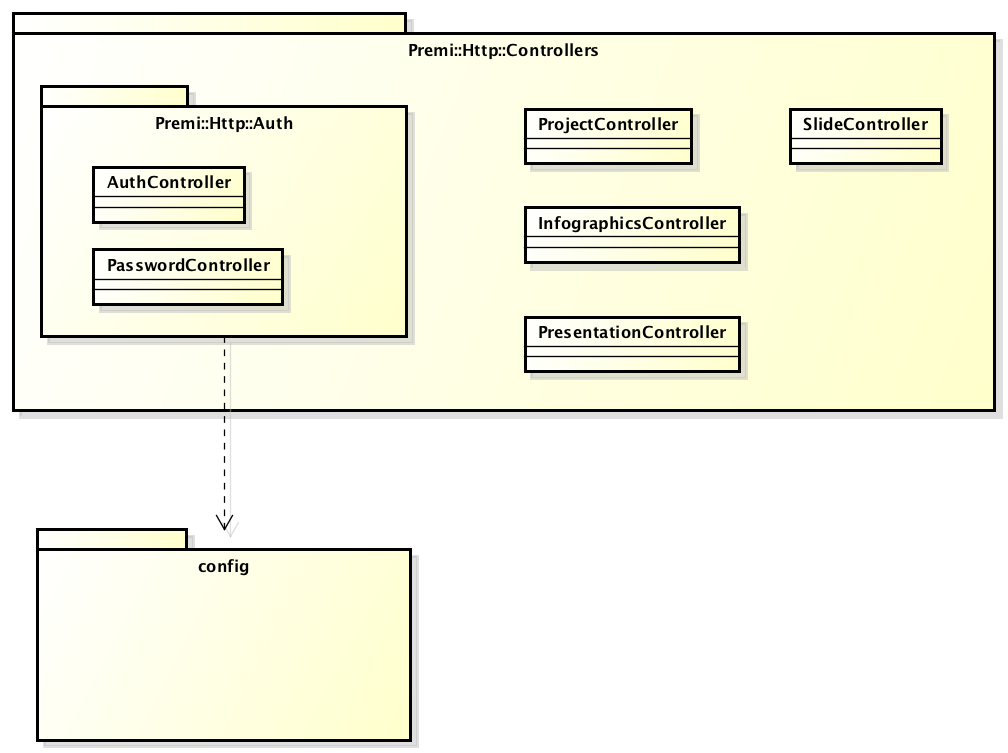
\includegraphics[width=0.9\linewidth]{img/premi_http_controllers}
		\caption[Premi::Http::Controllers]{Premi::Http::Controllers}
	\end{figure}
	Il package contiene le componenti che gestiscono la parte controller del lato \gls{back-end} dell'applicazione. 
	Sono presenti i controller per il progetto e i suoi componenti. È presente inoltre il package Auth che gestisce la parte di registrazione, autenticazione e recupero password dell'utente. 

	\subsubsection*{Package contenuti}
		\begin{itemize}
			\item Premi::Http::Auth
		\end{itemize}
	\subsubsection*{Classi contenute}
		\begin{itemize}
			\item Premi::Http::Controllers::ProjectController;
			\item Premi::Http::Controllers::InfographicController;
			\item Premi::Http::Controllers::Presentation;
			\item Premi::Http::Controllers::SlideController.
		\end{itemize}
		
	
	\subsubsection*{Premi::Http::Controllers::Auth}
		\subsubsection*{Informazioni sul package}
		\begin{figure}[h]
			\centering
			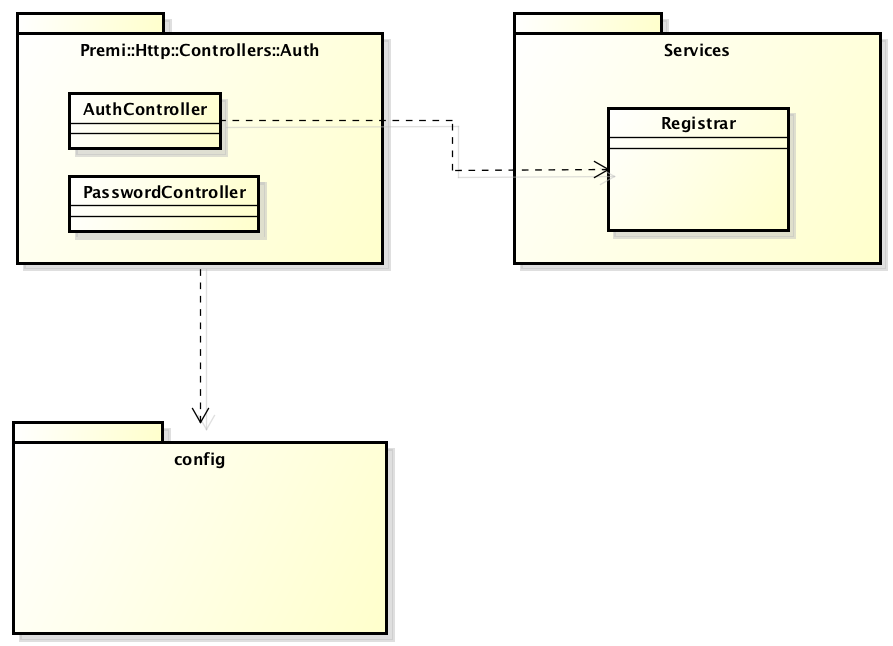
\includegraphics[width=0.9\linewidth]{img/premi_http_controllers_auth}
			\caption[Premi::Http::Controllers::Auth]{Premi::Http::Controllers::Auth}
			\label{fig:premi_http_controllers_auth}
		\end{figure}
	Laravel utilizza un semplice meccanismo di autenticazione. I file di configurazioni già documentate si trovano all'interno del package \textbf{config} che servono a ottimizzare il comportamento del servizio di autenticazione.		
	\subsubsection*{Classi contenute}
		\begin{itemize}
			\item Premi::Http::Auth::AuthController:
				\begin{itemize}
					\item \textbf{Descrizione}: AuthController gestisce le registrazioni di nuovi utenti e i loro accessi.
				\end{itemize}
			\item Premi::Http::Auth::PasswordController:
				\begin{itemize}
					\item \textbf{Descrizione:} PasswordController contiene la logica per aiutare gli utenti per il reset della password.
				\end{itemize}
		\end{itemize}
	Ognuno di questi controller usa un \gls{trait} che include i loro metodi necessari.\\
	Per modificare i campi del form necessari quando un nuovo utente si registra, è possibile farlo modificando la classe Services::Registrar. Questa classe è responsabile per la creazione e validazione dei nuovi utenti. Il metodo validator di Registrar contiene le regole di validazione per i nuovi utenti, mentre il metodo create di Registrar è responsabile della creazione di un nuovo record User nel database. Registrar è chiamato da AuthController tramite dei metodi contenuti nel \gls{trait} AuthenticatesAndRegistersUsers.
			
	\subsubsection*{Premi::Http::ProjectController}
			\begin{itemize}
				\item \textbf{Descrizione}: Classe che gestisce le operazioni e la logica riguardante la gestione e la modifica di un progetto;
			\end{itemize}
			
   \subsubsection*{Premi::Http::PresentationController}
			\begin{itemize}
				\item \textbf{Descrizione}: Classe che gestisce le operazioni e la logica riguardante la gestione e la modifica di una presentazione;
			\end{itemize}
			
	\subsubsection*{Premi::Http::InfographicsController}
			\begin{itemize}
				\item \textbf{Descrizione}: Classe che gestisce le operazioni e la logica riguardante la gestione e la modifica di un'\gls{infografica};
			\end{itemize}
			
	\subsubsection*{Premi::Http::SlideController}
			\begin{itemize}
				\item \textbf{Descrizione}: classe che gestisce le operazioni e la logica riguardante la gestione e la modifica di una \gls{slide};
			\end{itemize}
		
\newpage
\subsection{Premi::Http::Middleware}
\begin{figure}[h]
\centering
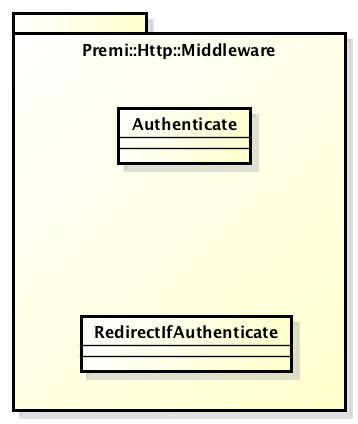
\includegraphics[width=0.7\linewidth]{img/premi_http_middleware}
\caption[Premi::Http::Middleware]{Premi::Http::Middleware}
\label{fig:premi_http_middleware}
\end{figure}

	\subsubsection*{Informazioni sul package}
	I middleware forniscono un meccanismo molto conveniente di filtraggio delle richieste HTTP in entrata.
	\subsubsection*{Classi contenute}
		\begin{itemize}
			\item \textbf{Premi::Http::Middleware::Autheticate:} verifica se l'utente dell'applicazione ha effettuato l'accesso correttamente;
			\item \textbf{Premi::Http::Middleware::RedirectIfAutheticate:} nel caso in cui il controllo precedente ha dato una risposta negativa, il middleware effettua un redirect verso la schermata di login. In caso contrario, invece, tutto prosegue normalmente.
		\end{itemize}
		
\newpage
\subsection{Premi::Http::Request}
\begin{figure}[h]
\centering
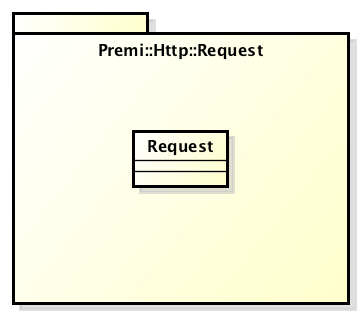
\includegraphics[width=0.7\linewidth]{img/premi_http_request}
\caption[Premi::Http::Request]{Premi::Http::Request}
\label{fig:premi_http_request}
\end{figure}
	\subsubsection*{Informazione sul package}
	La facade Request garantisce l'accesso alla richiesta corrente contenuta nel container.

	
%\subsection{Premi::Back-End::Logic-Tier::Controller::ComponentController}
%	\subsubsection*{Informazioni sul package}
%		\begin{figure}[h]
%			\centering
%			\includegraphics[width=0.9\linewidth]{img/back-end_logic-tier_controller_componentcontroller}
%			\caption[Premi::Back-End::Logic-Tier::Controller::ComponentController]{Premi::Back-End::Logic-Tier::Controller::ComponentController}
%		\end{figure}
%		Il package contiene le classi dei controller per la gestione degli elementi di una \gls{slide}.
%		
%	\subsubsection*{Classi contenute}
%	\begin{itemize}
%		\item Premi::Back-End::Logic-Tier::Controller::ComponentController::ComponentController:
%		\begin{itemize}
%			\item \textbf{Descrizione}: classe che gestisce le operazioni e la logica applicativa di tutti i componenti della \gls{slide};
%			\item \textbf{Relazioni con altre classi}:
%			\begin{itemize}
%				\item Premi::Back-End::Logic-Tier::Controller::FrontController.
%			\end{itemize}
%		\end{itemize}
%		
%		\item Premi::Back-End::Logic-Tier::Controller::ComponentController::RealTimeDataController:
%		\begin{itemize}
%			\item \textbf{Descrizione}: classe che gestisce le operazioni e la logica applicativa dei componenti per i dati real-time della \gls{slide};
%			\item \textbf{Relazioni con altre classi}:
%			\begin{itemize}
%				\item Premi::Back-End::Logic-Tier::Controller::ComponentController::ComponentController.
%			\end{itemize}
%		\end{itemize}
%		
%		\item Premi::Back-End::Logic-Tier::Controller::ComponentController::ChartController:
%		\begin{itemize}
%			\item \textbf{Descrizione}: classe che gestisce le operazioni e la logica applicativa dei componenti per i grafici della \gls{slide};
%			\item \textbf{Relazioni con altre classi}:
%			\begin{itemize}
%				\item Premi::Back-End::Logic-Tier::Controller::ComponentController::ComponentController.
%			\end{itemize}
%		\end{itemize}
%		
%		\item Premi::Back-End::Logic-Tier::Controller::ComponentController::ImageController:
%		\begin{itemize}
%			\item \textbf{Descrizione}: classe che gestisce le operazioni e la logica applicativa dei componenti per le immagini della \gls{slide};
%			\item \textbf{Relazioni con altre classi}:
%			\begin{itemize}
%				\item Premi::Back-End::Logic-Tier::Controller::ComponentController::ComponentController.
%			\end{itemize}
%		\end{itemize}
%		
%		\item Premi::Back-End::Logic-Tier::Controller::ComponentController::TableController:
%		\begin{itemize}
%			\item \textbf{Descrizione}: classe che gestisce le operazioni e la logica applicativa dei componenti per le tabelle della \gls{slide};
%			\item \textbf{Relazioni con altre classi}:
%			\begin{itemize}
%				\item Premi::Back-End::Logic-Tier::Controller::ComponentController::ComponentController.
%			\end{itemize}
%		\end{itemize}
%		
%		\item Premi::Back-End::Logic-Tier::Controller::ComponentController::TextController:
%		\begin{itemize}
%			\item \textbf{Descrizione}: classe che gestisce le operazioni e la logica applicativa dei componenti per le caselle di testo della \gls{slide};
%			\item \textbf{Relazioni con altre classi}:
%			\begin{itemize}
%				\item Premi::Back-End::Logic-Tier::Controller::ComponentController::ComponentController.
%			\end{itemize}
%		\end{itemize}
%	\end{itemize}
%	

\newpage
\subsection{Premi::Model}
	\subsubsection*{Informazioni sul package}
\begin{figure}[h]
\centering
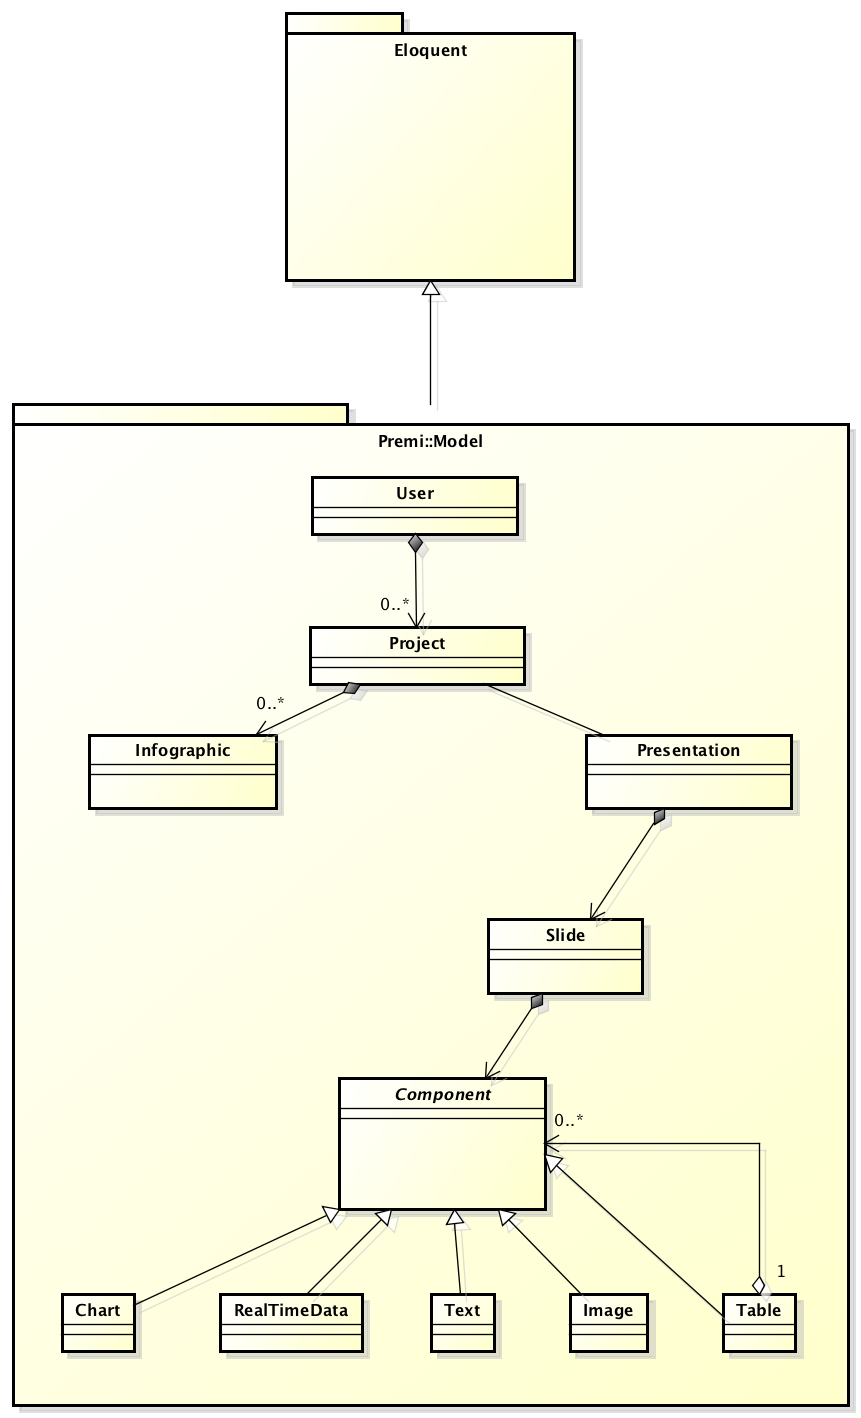
\includegraphics[width=0.7\linewidth]{img/premi_http_model}
\caption[Premi::Model]{Premi::Model}
\label{fig:premi_http_model}
\end{figure}
		Il package contiene la struttura delle classi di tutti i componenti dell'applicazione.
	
	\subsubsection*{Classi contenute}
	\begin{itemize}
		\item Premi::Model::User:
		\begin{itemize}
			\item \textbf{Descrizione:} classe contenente le informazioni di un utente.
		\end{itemize}
		\item Premi::Model::Project:
		\begin{itemize}
			\item \textbf{Descrizione}: classe base contenente le informazioni principali del progetto.
		\end{itemize}
			
		\item Premi::Model::Infographic:
		\begin{itemize}
			\item \textbf{Descrizione:} classe che rappresenta le infografiche associate a un progetto;
			\item \textbf{Relazione con altre classi}:
			\begin{itemize}
				\item Premi::Model::Project.
			\end{itemize}
		\end{itemize}
		
		\item Premi::Model::Presentation:
		\begin{itemize}
			\item \textbf{Descrizione:} classe che rappresenta la presentazione del progetto;
			\item \textbf{Relazione con altre classi}:
			\begin{itemize}
				\item Premi::Model::Project.
			\end{itemize}
		\end{itemize}
		
		\item Premi::Model::Slide:
		\begin{itemize}
			\item \textbf{Descrizione:} classe che rappresenta le \gls{slide} che compongono una presentazione;
			\item \textbf{Relazione con altre classi}:
			\begin{itemize}
				\item Premi::Model::Project.
			\end{itemize}
		\end{itemize}
		
		\item Premi::Model::Component:
		\begin{itemize}
			\item \textbf{Descrizione:} classe base che rappresenta i componenti di cui è formata una \gls{slide};
			\item \textbf{Relazione con altre classi}:
			\begin{itemize}
				\item Premi::Model::Project.
			\end{itemize}
		\end{itemize}
		
		\item Premi::Model::Chart:
		\begin{itemize}
			\item \textbf{Descrizione:} classe che rappresenta l'elemento "grafico" che può essere inserito in una \gls{slide};
			\item \textbf{Relazione con altre classi}:
			\begin{itemize}
				\item Premi::Model::Project.
			\end{itemize}
		\end{itemize}
		
		\item Premi::Model::RealTimeData:
		\begin{itemize}
			\item \textbf{Descrizione:} classe che rappresenta l'elemento "dati real-time" che può essere inserito in una \gls{slide};
			\item \textbf{Relazione con altre classi}:
			\begin{itemize}
				\item Premi::Model::Project.
			\end{itemize}
		\end{itemize}
		
		\item Premi::Model::Text:
		\begin{itemize}
			\item \textbf{Descrizione:} classe che rappresenta l'elemento "testo" che può essere inserito in una \gls{slide};
			\item \textbf{Relazione con altre classi}:
			\begin{itemize}
				\item Premi::Model::Project.
			\end{itemize}
		\end{itemize}
		
		\item Premi::Model::Image:
		\begin{itemize}
			\item \textbf{Descrizione:} classe che rappresenta l'elemento "immagine" che può essere inserito in una \gls{slide};
			\item \textbf{Relazione con altre classi}:
			\begin{itemize}
				\item Premi::Model::Project.
			\end{itemize}
		\end{itemize}
		
		\item Premi::Model::Table:
		\begin{itemize}
			\item \textbf{Descrizione:} classe che rappresenta l'elemento "tabella" che può essere inserito in una \gls{slide};
			\item \textbf{Relazione con altre classi}:
			\begin{itemize}
				\item Premi::Model::Project.
			\end{itemize}
		\end{itemize}
	\end{itemize}
	
\subsubsection*{Informazioni su Eloquent}
Eloquent è l'ORM(Object Relational Mapping) incluso in Laravel: un'implementazione di Active Record. Tutti i model estendono  Eloquent in modo da creare e gestire l'interazione con la collection.

\subsection{Data-Tier}
\begin{figure}[h]
\centering
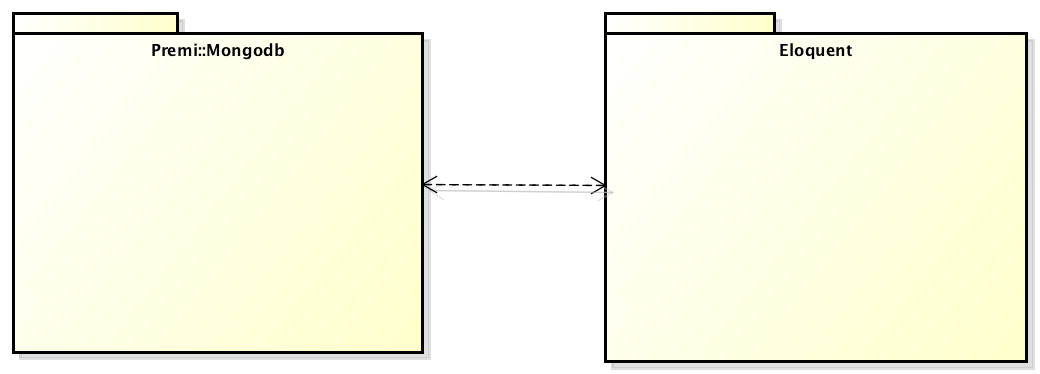
\includegraphics[width=0.7\linewidth]{img/premi_mongodb}
\caption[Premi::Mongodb]{Premi::Mongodb}
\label{fig:premi_mongodb}
\end{figure}
\subsubsection*{Informazioni sul package}
Ogni collection nel database trova una sua corrispondenza in un Model, il quale ha proprio il compito di gestire l'interazione con la collection stessa. Una volta definito il model se è pronti a selezionare un record, crearne di nuovi ed in generale lavorare con la collection. La sintassi è molto semplice: Laravel mette a disposizione le query tramite il Model Eloquent.
